Der allgemeine Ablauf der Anwendung kann in der Abbildung~\ref{fig:ProximetyUIFlow2} entnommen werden. Anschliessend folgen alle bisher definierten Fenster der Variante 2.

\setlength\fboxsep{0pt}
\setlength\fboxrule{0.5pt}

\def\guivartwo{bilder/guivariante2/}
\FloatBarrier
\begin{figure}[hp]
	\centering
	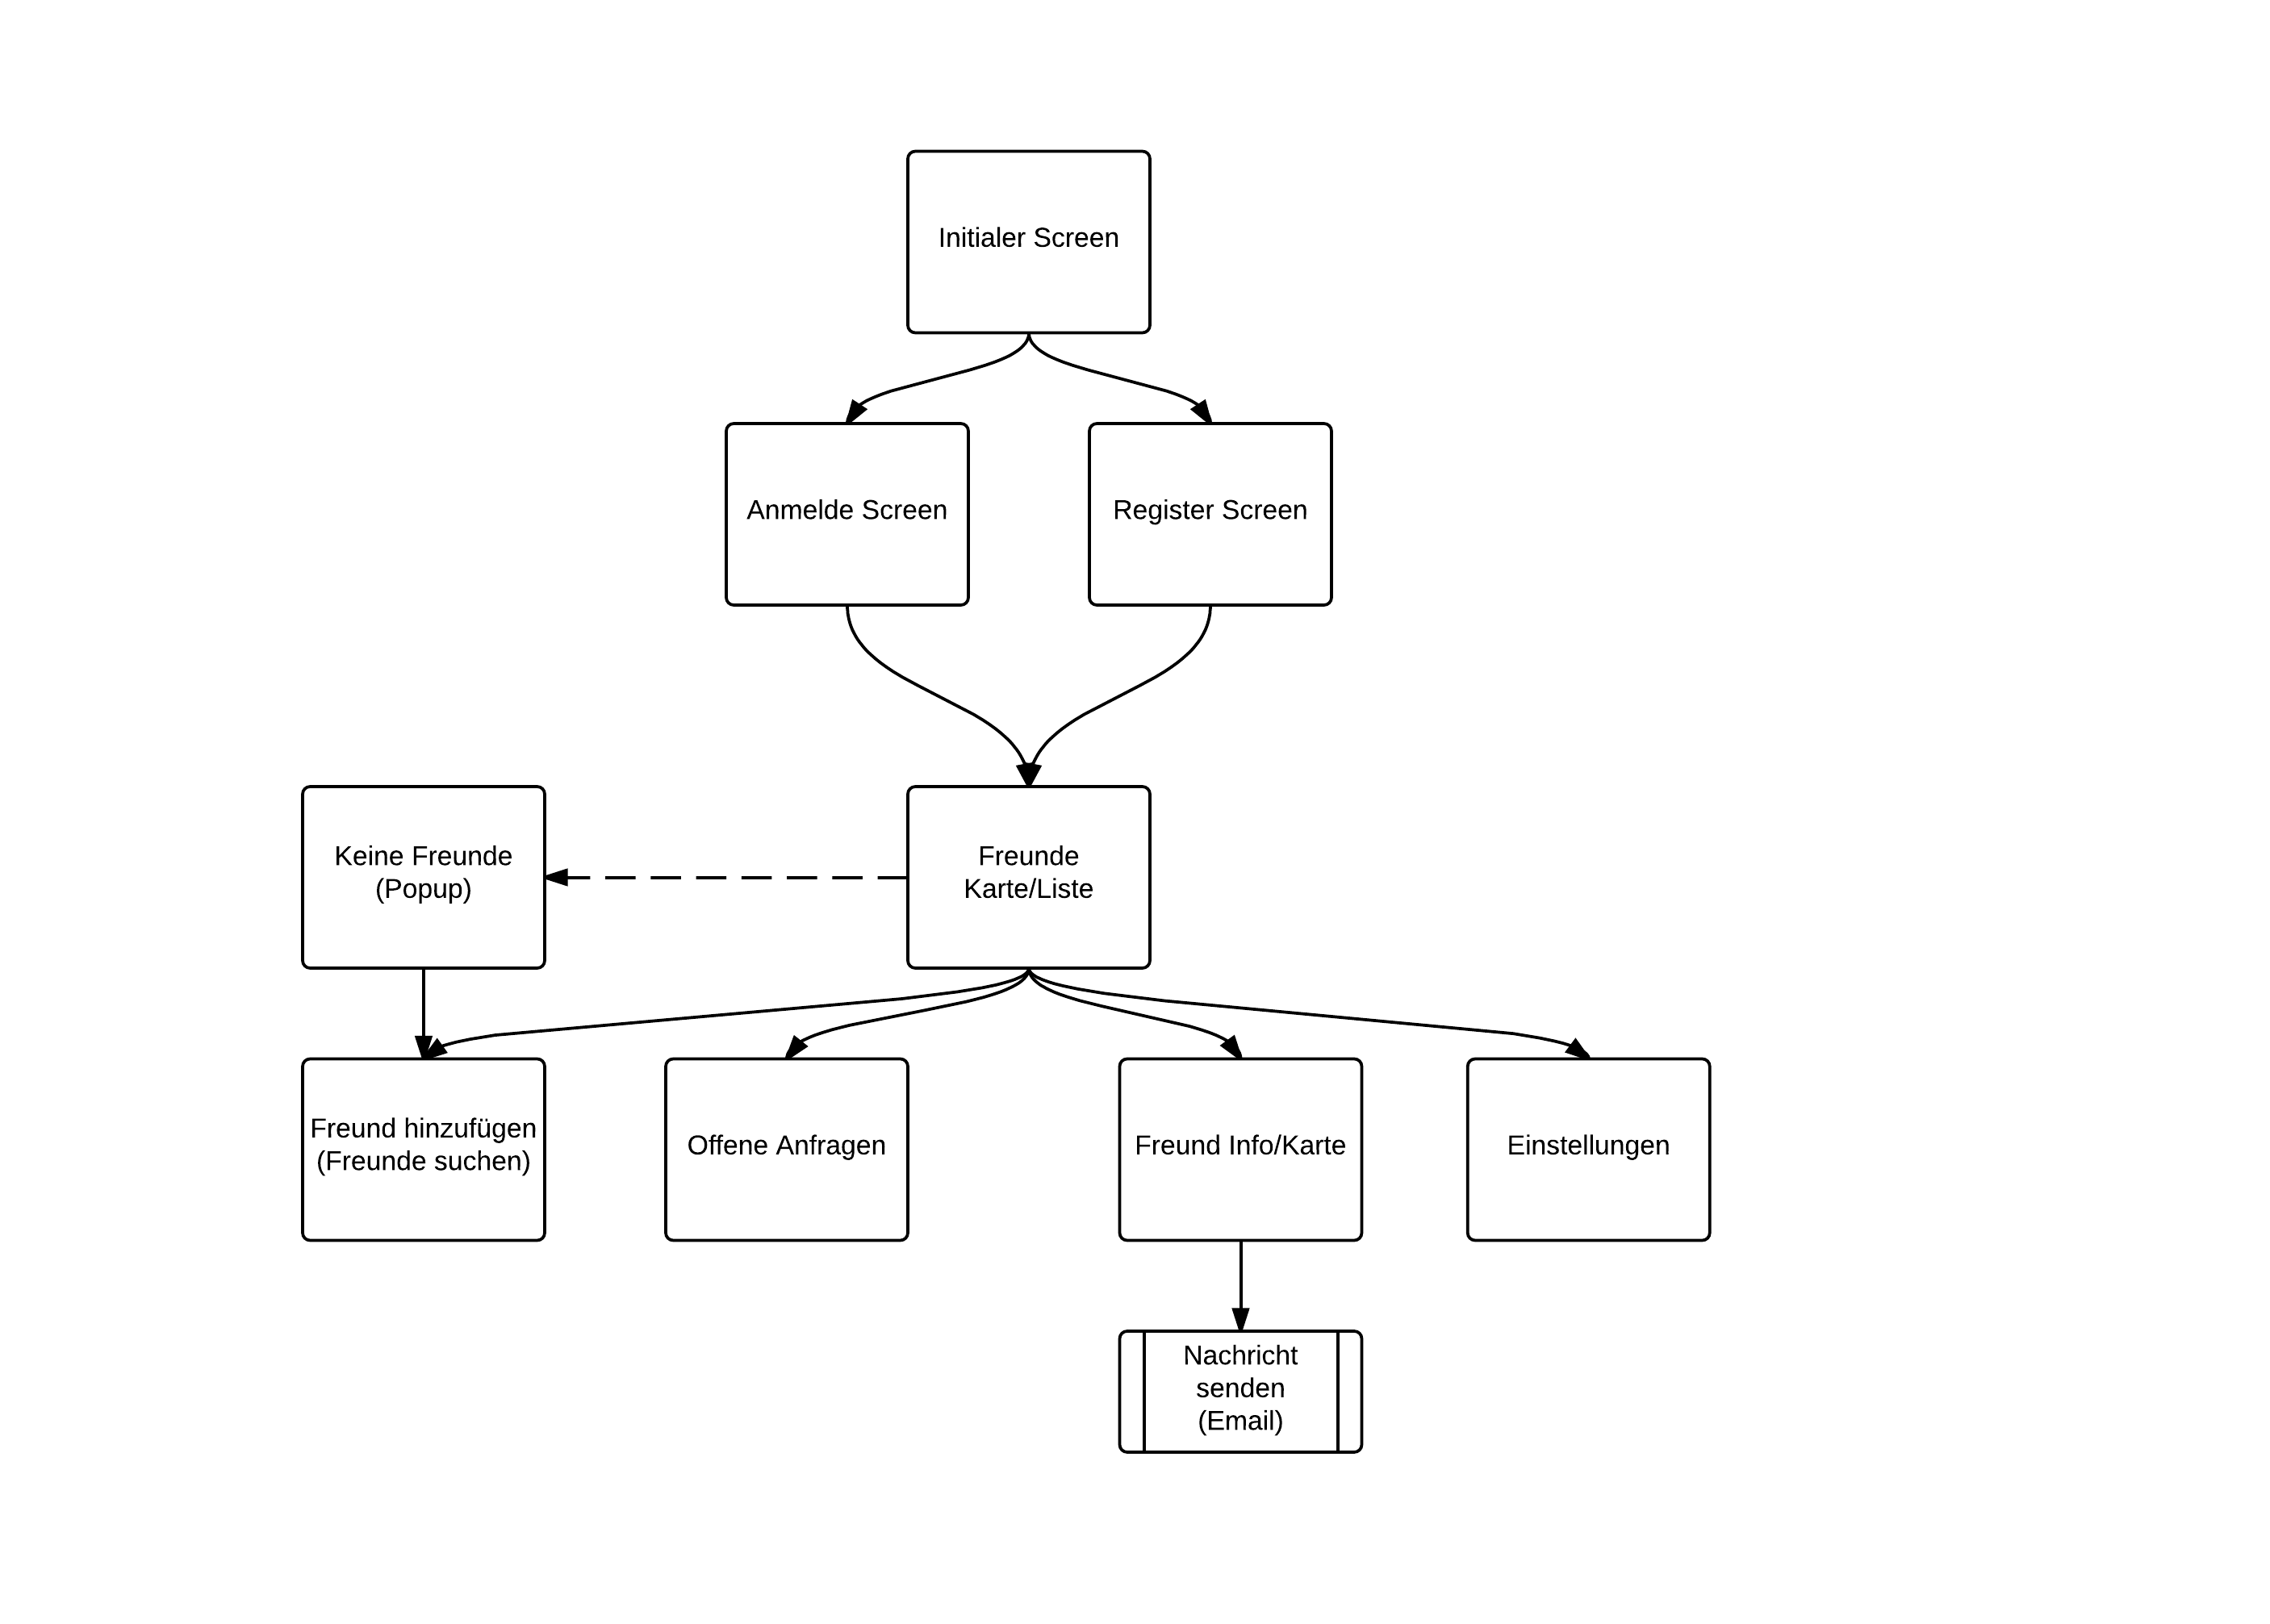
\includegraphics[scale=0.25]{ProximetyUIFlow2.png}
	\caption{Design Flow Diagramm}
	\label{fig:ProximetyUIFlow2}
\end{figure}
\FloatBarrier
\begin{figure}[H]
	\centering
	\begin{subfigure}[h]{0.3\textwidth}
		\fbox{\includegraphics[width=1\textwidth]{\guivartwo{Initialscreen.png}}}
		\caption{Initiales Fenster}
		\label{fig:initscreentwo}
	\end{subfigure}%
	\qquad %add desired spacing between images, e. g. ~, \quad, \qquad, \hfill etc.
	%(or a blank line to force the subfigure onto a new line)
	\begin{subfigure}[h]{0.3\textwidth}
		\fbox{\includegraphics[width=1\textwidth]{\guivartwo{Registrieren.png}}}
		\caption{Registrierungsfenster}
		\label{fig:registerscreentwo}
	\end{subfigure}
	\caption{Initialer und Registrierungsfenster}
\end{figure}
\begin{figure}[H]
	\centering
	\begin{subfigure}[h]{0.3\textwidth}
		\fbox{\includegraphics[width=1\textwidth]{\guivartwo{Anmelden.png}}}
		\caption{Anmeldung}
		\label{fig:logintwo}
	\end{subfigure}%
	\qquad %add desired spacing between images, e. g. ~, \quad, \qquad, \hfill etc.
	%(or a blank line to force the subfigure onto a new line)
	\begin{subfigure}[h]{0.3\textwidth}
		\fbox{\includegraphics[width=1\textwidth]{\guivartwo{Leere Freundesliste.png}}}
		\caption{Keine Kontakte}
		\label{fig:mainempty}
	\end{subfigure}
	\caption{Anmeldungs- und Hauptfenster (Ohne Kontakte)}
\end{figure}
\begin{figure}[H]
	\centering
	\begin{subfigure}[h]{0.3\textwidth}
		\fbox{\includegraphics[width=1\textwidth]{\guivartwo{Freunde - Liste.png}}}
		\caption{Hauptfenster (Liste)}
		\label{fig:mainlist}
	\end{subfigure}%
	\qquad %add desired spacing between images, e. g. ~, \quad, \qquad, \hfill etc.
	%(or a blank line to force the subfigure onto a new line)
	\begin{subfigure}[h]{0.3\textwidth}
		\fbox{\includegraphics[width=1\textwidth]{\guivartwo{Freunde - Karte.png}}}
		\caption{Hauptfenster (Karte)}
		\label{fig:mainmap}
	\end{subfigure}
	\caption{Hauptfenster in Listen- und Kartenansicht }
\end{figure}
\begin{figure}[H]
	\centering
	\begin{subfigure}[h]{0.3\textwidth}
		\fbox{\includegraphics[width=1\textwidth]{\guivartwo{Offene Anfragen.png}}}
		\caption{Offene Anfragen}
		\label{fig:openrequests}
	\end{subfigure}%
	\qquad %add desired spacing between images, e. g. ~, \quad, \qquad, \hfill etc.
	%(or a blank line to force the subfigure onto a new line)
	\begin{subfigure}[h]{0.3\textwidth}
		\fbox{\includegraphics[width=1\textwidth]{\guivartwo{Freund hinzufuegen.png}}}
		\caption{Freund hinzufügen}
		\label{fig:addfriend}
	\end{subfigure}
	\caption{Freundschatsanfragen stellen und beantworten }
\end{figure}
\begin{figure}[H]
	\centering
	\begin{subfigure}[h]{0.3\textwidth}
		\fbox{\includegraphics[width=1\textwidth]{\guivartwo{Freund - Details.png}}}
		\caption{Freund Details}
		\label{fig:frienddetails}
	\end{subfigure}%
	\qquad %add desired spacing between images, e. g. ~, \quad, \qquad, \hfill etc.
	%(or a blank line to force the subfigure onto a new line)
	\begin{subfigure}[h]{0.3\textwidth}
		\fbox{\includegraphics[width=1\textwidth]{\guivartwo{Freund - Karte.png}}}
		\caption{Freund Karte}
		\label{fig:friendmap}
	\end{subfigure}
	\caption{Detail- und Kartenansicht für Freund}
\end{figure}
\begin{figure}[H]
	\centering
	\begin{subfigure}[h]{0.3\textwidth}
		\fbox{\includegraphics[width=1\textwidth]{\guivartwo{Menu.png}}}
		\caption{Menu}
		\label{fig:menu}
	\end{subfigure}%
	\qquad %add desired spacing between images, e. g. ~, \quad, \qquad, \hfill etc.
	%(or a blank line to force the subfigure onto a new line)
	\begin{subfigure}[h]{0.3\textwidth}
		\fbox{\includegraphics[width=1\textwidth]{\guivartwo{Notification - Alarm.png}}}
		\caption{Benachrichtigung}
		\label{fig:loginscreenone}
	\end{subfigure}
	\caption{Menu und Benachrichtigung }
\end{figure}